\documentclass{article}
\usepackage{amsmath}
\usepackage{caratula}

\begin{document}

\titulo{SoftFPGA}
\subtitulo{Informe}

\fecha{\today}

\materia{Programación de softcores en FPGAs}
\grupo{ret = pop rip}

\integrante{Losiggio, Ignacio Esteban}{751/17}{iglosiggio@dc.uba.ar}
\integrante{Demartino, Francisco}{348/14}{email2@dominio.com}

\maketitle

\begin{abstract}
El siguiente informe detalla el trabajo de diseño, verificación e implementación llevado a cabo por Ignacio Losiggio y Francisco Demartino bajo el marco de la materia \emph{``Programación de Softcores en FPGAs"} dictada por David Alejandro González Márquez. El informe consiste en cuatro partes que corresponden a etapas del trabajo: diseño, implementación, evaluación en un simulador y construcción de software auxiliar para ayudar al desarrollo de programas. Aunque el trabajo realizado no sucedió con etapas tan marcadas creemos que esta forma de narrarlo da pié a un mejor informe.
\end{abstract}

\tableofcontents

\newpage

\section{ISA}

Nuestra arquitectura es de una máquina de 8-bits con dos interfaces de memoria:
\begin{itemize}
    \item \textbf{Datos:}  1kb, direccionable a 8bit (direcciones de 10 bits)
    \item \textbf{Código:} 1kb, direccionable a 16bit (direcciones de 9 bits)
\end{itemize}

La ISA posee 16 registros (\texttt{r0} a \texttt{rf}). Todos los registros pueden utilizarse para operación aritméticas y de acceso a memoria sin distinción.

Algunos registros son usados implícitamente dentro de varios mecanismos del procesador:
\begin{itemize}
    \item \texttt{r0}: siempre vale \texttt{0x00}
    \item \texttt{r8}: usado como destino implícito de las operaciones aritméticas y la instrucción \texttt{setcc}
    \item \texttt{r9}: offset de la próxima instrucción en el segmento de código actual
    \item \texttt{rc}: $\frac{\text{base}}{2}$ del segmento de código actual
    \item \texttt{rd}: $\frac{\text{base}}{4}$ del segmento de datos actual
    \item \texttt{rf}: siempre vale \texttt{0xFF}
\end{itemize}

Nuestro ensamblador soporta una serie de nombres alternativos o ``alias" que sugieren ciertos usos para los registros.

\begin{table}[h]
    \centering
    \begin{tabular}{c|c|c}
        \textbf{Registro} & \textbf{Aliases} & \textbf{Uso} \\
        \texttt{r0}       & \texttt{bh}      & black hole, siempre \texttt{0x00} \\
        \texttt{r1}       & \texttt{a}       & propósito general \\
        \texttt{r2}       & \texttt{b}       & propósito general \\
        \texttt{r3}       & \texttt{c}       & propósito general \\
        \texttt{r4}       & \texttt{d}       & propósito general \\
        \texttt{r5}       & \texttt{e}       & propósito general \\
        \texttt{r6}       & \texttt{f}       & propósito general \\
        \texttt{r7}       & \texttt{g}       & propósito general \\
        \texttt{r8}       & \texttt{fl}      & flags (\texttt{S\_\_\_CNVZ}) \\
        \texttt{r9}       & \texttt{ip} \texttt{rip} \texttt{pc} 
                                             & instruction pointer \\
        \texttt{ra}       & \texttt{sp}      & stack pointer \\
        \texttt{rb}       & \texttt{juanca}  & scratch register \\
        \texttt{rc}       & \texttt{cs}      & code segment \\
        \texttt{rd}       & \texttt{ds}      & data segment \\
        \texttt{re}       & \texttt{lr}      & link register \\
        \texttt{rf}       & \texttt{wh}      & white hole, siempre \texttt{0xFF} \\
    \end{tabular}
    \caption{Nombres y usos comunes de los registros}
\end{table}

\subsection{Macros}
Nuestro lenguaje ensamblador es procesado por \texttt{cpp}, el preprocesador del lenguaje C. En los programas entregados hacemos uso de varios macros ``estándar" para ayudar a la legibilidad de los mismos. Dado que el preprocesador elimina todos los comentarios válidos en el lenguaje C (\texttt{/* comentario */} y \texttt{// comentario}) el uso del mismo nos proporciona una forma sencilla de documentar nuestro código sin tener que implementarla en nuestro ensamblador.

\subsubsection{\texttt{calli(addr)}}
\begin{verbatim}
// llamada a subrutina con dirección inmediata
push(lr)
movi lr addr
xchg lr ip
pop(lr)
\end{verbatim}
\subsubsection{\texttt{callr(reg)}}
\begin{verbatim}
// llamada a subrutina con indirección via registro
push(lr)
movr lr reg
xchg lr ip
pop(lr)
\end{verbatim}
\subsubsection{\texttt{ret}}
\begin{verbatim}
// retorno de subrutina
movr ip lr
\end{verbatim}
\subsubsection{\texttt{jmpi(addr)}}
\begin{verbatim}
// salto a dirección inmediata
movi ip addr
\end{verbatim}
\subsubsection{\texttt{jmpr(reg)}}
\begin{verbatim}
// salto indirecto via registro
movr ip reg
\end{verbatim}
\subsubsection{\texttt{push(reg)}}
\begin{verbatim}
// push del valor de un registro a la pila
storer [sp] reg
add sp wh
\end{verbatim}
\subsubsection{\texttt{pop(reg)}}
\begin{verbatim}
// pop de la pila a un registro
sub sp wh
loadr reg [sp]
\end{verbatim}

\subsection{Instrucciones}

La mayoría de las instrucciones de nuestra ISA son \emph{``skipeables''}. Si en los flags del procesador el bit de skip está en 1, entonces toda instrucción \emph{``skipeable''} que también lo tenga alto se ejecutará como si fuera un \texttt{nop}. La representación del bit de skip en nuestro lenguaje ensamblador es por medio del prefijo \texttt{maybe}. Éste es el único mecanismo de ejecución condicional que nuestro procesador posee (por ejemplo: un salto condicional es \texttt{maybe add ip <reg>}).

En las siguientes secciones, el Encoding de cada instrucción representa bits en little endian (el de más a la derecha es el menos significativo). Un guión bajo (\texttt{\_}) indica que el valor en esa posición no se usa.

\subsubsection{\texttt{storei [imm10] r4}}
\begin{itemize}
    \item \textbf{Encoding:} \texttt{11 AAAAAAAAAA RRRR}
    \item \textbf{Operación:} Escribe \texttt{r4} a la dirección de memoria indicada por \texttt{imm10}
    \item No es skipeable
\end{itemize}

\subsubsection{\texttt{loadi r4 [imm10]}}
\begin{itemize}
    \item \textbf{Encoding:} \texttt{01 AAAAAAAAAA RRRR}
    \item \textbf{Operación:} Escribe en \texttt{r4} el valor encontrado en la dirección de memoria indicada por \texttt{imm10}
    \item No es skipeable
\end{itemize}

\subsubsection{\texttt{movi r4 imm8}}
\begin{itemize}
    \item \textbf{Encoding:} \texttt{0111 DDDDDDDD RRRR}
    \item \textbf{Operación:} Escribe en \texttt{r4} el valor \texttt{imm8}
    \item No es skipeable
\end{itemize}

\subsubsection{\texttt{sl r4 imm3}}
\begin{itemize}
    \item \textbf{Encoding:} \texttt{0110 111 S \_III RRRR}
    \item \textbf{Operación:} Multiplica \texttt{r4} por 2 \texttt{imm8} veces
    \item \textbf{Flags:}
        \begin{itemize}
            \item \textbf{c:} Valor del último bit que se shifteó \emph{``afuera''} de \texttt{r4}
            \item \textbf{n:} 1 si el bit de signo del resultado es 1, 0 sino
            \item \textbf{v:} Siempre cero
            \item \textbf{z:} 1 si el resultado es 0, 0 sino
        \end{itemize}
\end{itemize}
    
\subsubsection{\texttt{sra r4 imm3}}
\begin{itemize}
    \item \textbf{Encoding:} \texttt{0110 110 S 0III RRRR}
    \item \textbf{Operación:} Divide \texttt{r4} por 2 \texttt{imm8} veces (realiza división con signo)
    \item \textbf{Flags:}
        \begin{itemize}
            \item \textbf{c:} Siempre creo
            \item \textbf{n:} 1 si el bit de signo del resultado es 1, 0 sino
            \item \textbf{v:} Siempre cero
            \item \textbf{z:} 1 si el resultado es 0, 0 sino
        \end{itemize}
\end{itemize}

\subsubsection{\texttt{srl r4 imm3}}
\begin{itemize}
    \item \textbf{Encoding:} \texttt{0110 110 S 1III RRRR}
    \item \textbf{Operación:} Divide \texttt{r4} por 2 \texttt{imm8} veces (realiza división sin signo)
    \item \textbf{Flags:}
    \begin{itemize}
        \item \textbf{c:} Siempre cero
        \item \textbf{n:} 1 si el bit de signo del resultado es 1, 0 sino
        \item \textbf{v:} Siempre cero
        \item \textbf{z:} 1 si el resultado es 0, 0 sino 
    \end{itemize}
\end{itemize}

\subsubsection{\texttt{cmp r4a r4b}}
\begin{itemize}
    \item \textbf{Encoding:} \texttt{0110 101 S RRRR RRRR}
    \item \textbf{Operación:} Modifica los flags de acuerdo al resultado de \texttt{r4a} - \texttt{r4b}
    \item \textbf{Flags:}
        \begin{itemize}
            \item \textbf{c:} 1 si \texttt{r4b} era mayor a \texttt{r4a} (interpretación sin signo)
            \item \textbf{n:} 1 si el bit de signo del resultado es 1, 0 sino
            \item \textbf{v:} 1 si el resultado no es representable en 8 bits (interpretación con signo)
            \item \textbf{z:} 1 si el resultado es 0, 0 sino
        \end{itemize}
\end{itemize}

\subsubsection{\texttt{sub r4a r4b}}
\begin{itemize}
    \item \textbf{Encoding:} \texttt{0110 100 S RRRR RRRR}
    \item \textbf{Operación:} \texttt{r4a} $\Leftarrow$ \texttt{r4a} - \texttt{r4b}
    \item \textbf{Flags:}
        \begin{itemize}
            \item \textbf{c:} 1 si \texttt{r4b} era mayor a \texttt{r4a} (interpretación sin signo)
            \item \textbf{n:} 1 si el bit de signo del resultado es 1, 0 sino
            \item \textbf{v:} 1 si el resultado no es representable en 8 bits (interpretación con signo)
            \item \textbf{z:} 1 si el resultado es 0, 0 sino
        \end{itemize}
\end{itemize}

\subsubsection{\texttt{add r4a r4b}}
\begin{itemize}
    \item \textbf{Encoding:} \texttt{0110 011 S RRRR RRRR}
    \item \textbf{Operación:} \texttt{r4a} $\Leftarrow$ \texttt{r4a} - \texttt{r4b}
    \item \textbf{Flags:}
        \begin{itemize}
            \item \textbf{c:} 1 si el resultado de la suma no es representable en 8 bits (interpretación sin signo)
            \item \textbf{n:} 1 si el bit de signo del resultado es 1, 0 sino
            \item \textbf{v:} 1 si el resultado no es representable en 8 bits (interpretación con signo)
            \item \textbf{z:} 1 si el resultado es 0, 0 sino
        \end{itemize}
\end{itemize}
  
\subsubsection{\texttt{xor r4a r4b}}
\begin{itemize}
    \item \textbf{Encoding:} \texttt{0110 010 S RRRR RRRR}
    \item \textbf{Operación:} \texttt{r4a} $\Leftarrow$ \texttt{r4a} \^{} \texttt{r4b}
    \item \textbf{Flags:}
        \begin{itemize}
            \item \textbf{c:} Siempre cero
            \item \textbf{n:} 1 si el bit de signo del resultado es 1, 0 sino
            \item \textbf{v:} Siempre cero
            \item \textbf{z:} 1 si el resultado es 0, 0 sino
        \end{itemize}
\end{itemize}

\subsubsection{\texttt{or r4a r4b}}
\begin{itemize}
    \item \textbf{Encoding:} \texttt{0110 001 S RRRR RRRR}
    \item \textbf{Operación:} \texttt{r4a} $\Leftarrow$ \texttt{r4a} \textbar{} \texttt{r4b}
    \item \textbf{Flags:}
        \begin{itemize}
            \item \textbf{c:} Siempre cero
            \item \textbf{n:} 1 si el bit de signo del resultado es 1, 0 sino
            \item \textbf{v:} Siempre cero
            \item \textbf{z:} 1 si el resultado es 0, 0 sino
        \end{itemize}
\end{itemize}

\subsubsection{\texttt{and r4a r4b}}
\begin{itemize}
    \item \textbf{Encoding:} \texttt{0110 000 S RRRR RRRR}
    \item \textbf{Operación:} \texttt{r4a} $\Leftarrow$ \texttt{r4a} \& \texttt{r4b}
    \item \textbf{Flags:}
        \begin{itemize}
            \item \textbf{c:} Siempre cero
            \item \textbf{n:} 1 si el bit de signo del resultado es 1, 0 sino
            \item \textbf{v:} Siempre cero
            \item \textbf{z:} 1 si el resultado es 0, 0 sino
        \end{itemize}
\end{itemize}

\subsubsection{\texttt{setcc op cond}}
\begin{itemize}
    \item \textbf{Encoding:} \texttt{0101 OOO S MMMM FFFF}
    \item \textbf{Operación:} \texttt{flags[7]} $\Leftarrow$ \texttt{op}(\texttt{flags[7]}, \texttt{cond})
        \begin{itemize}
            \item \textbf{Códigos de operación:}
                \begin{itemize}
                    \item \texttt{000}: Set to zero
                    \item \texttt{001}: NOR
                    \item \texttt{010}: XOR
                    \item \texttt{011}: NAND
                    \item \texttt{100}: AND
                    \item \texttt{101}: XNOR
                    \item \texttt{110}: OR
                    \item \texttt{111}: Set to one
                \end{itemize}
            \item \textbf{Condición:} La condición se describe con una cadena de texto con la forma \texttt{[cC][nN][vV][zZ]}. Las letras minúsculas describen bits de los flags que deben ser cero mientras que las mayúsculas bits que deben ser unos. Sólo se verificará el valor de las letras que formen parte de la condición. \emph{Ejemplo:} \texttt{cNv} es una condición que sólo se hará cierta si el carry es 0, el overflow es cero y el flag de
            negativo es 1.
        \end{itemize}
        \item \textbf{Flags:}
        \begin{itemize}
            \item \textbf{s:} Es el flag que estamos afectando (\texttt{flags[7]})
        \end{itemize}
  \end{itemize}
      
\subsubsection{\texttt{storer [r4b] r4a}}
\begin{itemize}
    \item \textbf{Encoding:} \texttt{0011 \_\_\_ S RRRR RRRR}
    \item \textbf{Operación:} \texttt{[(ds << 2) + r4b]} = \texttt{r4a}
\end{itemize}

\subsubsection{\texttt{loadr r4a [r4b]}}
\begin{itemize}
    \item \textbf{Encoding:} \texttt{0010 \_\_\_ S RRRR RRRR}
    \item \textbf{Operación:} \texttt{r4a} = \texttt{[(ds << 2) + r4b]}
\end{itemize}

\subsubsection{\texttt{xchg r4a r4b}}
\begin{itemize}
    \item \textbf{Encoding:} \texttt{0001 \_\_\_ S RRRR RRRR}
    \item \textbf{Operación:} \texttt{r4a}, \texttt{r4b} = \texttt{r4b}, \texttt{r4a}
\end{itemize}

\subsubsection{\texttt{movr r4a r4b}}
\begin{itemize}
    \item \textbf{Encoding:} \texttt{0000 \_\_\_ S RRRR RRRR}
    \item \textbf{Operación:} \texttt{r4a} = \texttt{r4b}
\end{itemize}

\section{Implementación}
Nuestra implementación se divide en 8 componentes. Cada componente es testeado de manera aislada y luego tres tests nos permiten evaluar el procesador con todas sus partes debidamente integradas.

\subsection{\texttt{alu.v}}
\begin{verbatim}
module alu(
    input  [2:0] op,          
    input  [7:0] a,              
    input  [7:0] b,             
    input        shift_logical,  
    input  [2:0] shift_imm,   
      
    output [7:0] r,           
    output [3:0] flags         
);
\end{verbatim}
En \texttt{alu.v} se implementa la unidad aritmético-lógica de nuestro procesador. El componente es completamente combinacional. El módulo recibe la operación a realizar (\texttt{op}, \texttt{shift\_logical}) y sus operandos (\texttt{a}, \texttt{b}, \texttt{shift\_imm}) como entrada y emite el valor resultado (\texttt{r}) y las flags asociadas (\texttt{flags}) como salida. Es importante notar que las flags asociadas son sólo cuatro (carry, negative, overflow y zero) pese a que el registro de flags es de 8 bits.

\subsection{\texttt{registers.v}}
\begin{verbatim}
module registers(
    input        clk,
    input        rst,
    input  [3:0] sel_read_a,
    input  [3:0] sel_read_b,
    input        exchange_a_b,
    input        en_write_reg,
    input  [3:0] sel_write_reg,
    input  [7:0] data_write_reg,
    input        en_write_flags,
    input  [7:0] data_write_flags,
    input        en_write_ip,
    input  [7:0] data_write_ip,

    output [7:0] r_read_a,
    output [7:0] r_read_b,
    output [7:0] r_flags,
    output [7:0] r_ip,
    output [7:0] r_cs,
    output [7:0] r_ds
);
\end{verbatim}
En \texttt{registers.v} se implementa nuestro banco de 16 registros. El mismo posee dos puertos de lectura (\texttt{sel\_read\_a}, \texttt{r\_read\_a} y \texttt{sel\_read\_b}, \texttt{r\_read\_b}) y uno de escritura (\texttt{en\_write\_reg}, \texttt{sel\_write\_reg}, \texttt{data\_write\_reg}). Adicionalmente los registros \texttt{r8} (\texttt{flags}), \texttt{r9} (\texttt{ip}), \texttt{rc} (\texttt{cs}) y \texttt{rd} (\texttt{ds}) se encuentran siempre expuestos para que el procesador pueda hacer uso de ellos.

Finalmente nuestro banco de registros implementa la instrucción \texttt{xchg} por medio de la señal \texttt{exchange\_a\_b} la cual causa un intercambio entre los registros seleccionados por los dos puertos de lectura. Las escrituras por medio de intercambios o del puerto de escritura toman precedencia sobre los puertos de escritura dedicados (\texttt{ip}, \texttt{flags}).

\subsection{\texttt{io.v}}
\begin{verbatim}
module io(
    input        clk,

    input        en_store,
    input  [9:0] addr_store,
    input  [7:0] data_store,

    input        en_load,
    input  [9:0] addr_load,
    output [7:0] data_load,
    
    input  [7:0] io_input,
    output [7:0] io_output,

    output       mem_en_load,
    output       mem_en_store
);
\end{verbatim}
En \texttt{io.v} se implementa la lógica de interacción con el mundo exterior. El módulo de \texttt{io} recibe las señales propias de una carga a memoria y sólo habilita la misma si la dirección en cuestión no es una de las reservadas (\texttt{0x3FF} y \texttt{0x3FE}). Durante cada clock \texttt{io.v} actualiza su registro interno del puerto de entrada y expone constantemente el último valor escrito al puerto de salida.

\subsection{\texttt{setcc\_logic.v}}
\begin{verbatim}
module setcc_logic(
    input previous_s,
    input [2:0] op,
    input [3:0] mask,
    input [3:0] expected_flags,
    input [3:0] current_flags,

    output s
);
\end{verbatim}
\texttt{setcc\_logic.v} implementa la lógica necesaria para la instrucción \texttt{setcc}. Es un componente completamente combinacional.

\subsection{\texttt{ir.v}}
\begin{verbatim}
module ir(
    input  [15:0] data,
    input         skip,

    output [3:0] op_code,
    output [2:0] subop_code,
    output [9:0] addr,
    output [7:0] imm,
    output [3:0] sel_ra,
    output [3:0] sel_rb,
    output       shift_logical,
    output [2:0] shift_imm,
    output [3:0] setcc_mask,
    output [3:0] setcc_expected
);
\end{verbatim}
\texttt{ir.v} implementa la decodificación de las instrucciones de nuestra ISA. Es un componente completamente combinacional. El mecanismo de ejecución condicional se implementa en este componente: cuando una instrucción \emph{skipeable} es fetcheada el módulo emitirá las señales necesarias para causar un \texttt{nop} (\texttt{mov bh, bh}) si la señal \texttt{skip} se encuentra activa.

\subsection{\texttt{core.v}}
\begin{verbatim}
module core(
    input         clk,
    input         rst,

    input  [15:0] instruction,
    input  [7:0]  mem_load,

    output        mem_en_store,
    output        mem_en_load,
    output [7:0]  mem_store,
    output [9:0]  mem_addr,
    output [8:0]  instruction_addr,

    input  [7:0]  io_input,
    output [7:0]  io_output
);
\end{verbatim}

\texttt{core.v} integra todos los componentes anteriores para construir nuestro núcleo. Las señales de control se encuentran (lamentablemente) implementadas aquí. La interfaz de nuestro núcleo es sencilla:
\begin{itemize}
    \item Un bus de código de 16 bits: (\texttt{instruction\_addr}, \texttt{instruction})
    \item Un bus de datos de 8 bits: (\texttt{mem\_addr}, \texttt{mem\_load}, \texttt{mem\_store}, \texttt{mem\_en\_store}, \texttt{mem\_en\_load})
    \item Un puerto de I/O de entrada de 8 bits: \texttt{io\_input}
    \item Un puerto de I/O de salida de 8 bits: \texttt{io\_output}
\end{itemize}

\subsection{\texttt{mem.v}}
\begin{verbatim}
module mem(
    input        clk,

    input        en_store,
    input  [9:0] addr_store,
    input  [7:0] data_store,

    input        en_load,
    input  [9:0] addr_load,
    output [7:0] data_load
);
```
\end{verbatim}
\texttt{mem.v} implementa la memoria de datos de 1kb. Posee un puerto de lectura (\texttt{en\_load}, \texttt{addr\_load}, \texttt{data\_load}) y uno de escritura (\texttt{en\_store}, \texttt{addr\_store}, \texttt{data\_store}).

\subsection{\texttt{plaquita.v}}
\begin{verbatim}
module plaquita(
    input        sysclk,
    input  [3:0] sw,
    input  [3:0] btn,
    output [3:0] led
);
\end{verbatim}
\texttt{plaquita.v} implementa nuestro core en la FPGA. El puerto de entrada del core es la combinación de los botones (\texttt{btn}) y los switches (\texttt{sw}) disponibles en la placa mientras que a la salida sólo conectamos los cuatro bits menos significativos a los leds (\texttt{led}) de la placa.

\subsection{Ciclo de instrucción}
La máquina está construida de forma que \texttt{core.v} ejecuta una instrucción por ciclo. Por problemas del diseño actual el clock máximo soportado es menor al clock de la placa que utilizamos en la materia. Por esto la implementación entregada hace uso del \emph{``Clocking wizard"} provisto por Xilinx para generar un clock mucho menor (10MHz) en el cuál nuestro diseño funcione.

\subsection{Datapath}

\begin{figure}
    \centering
    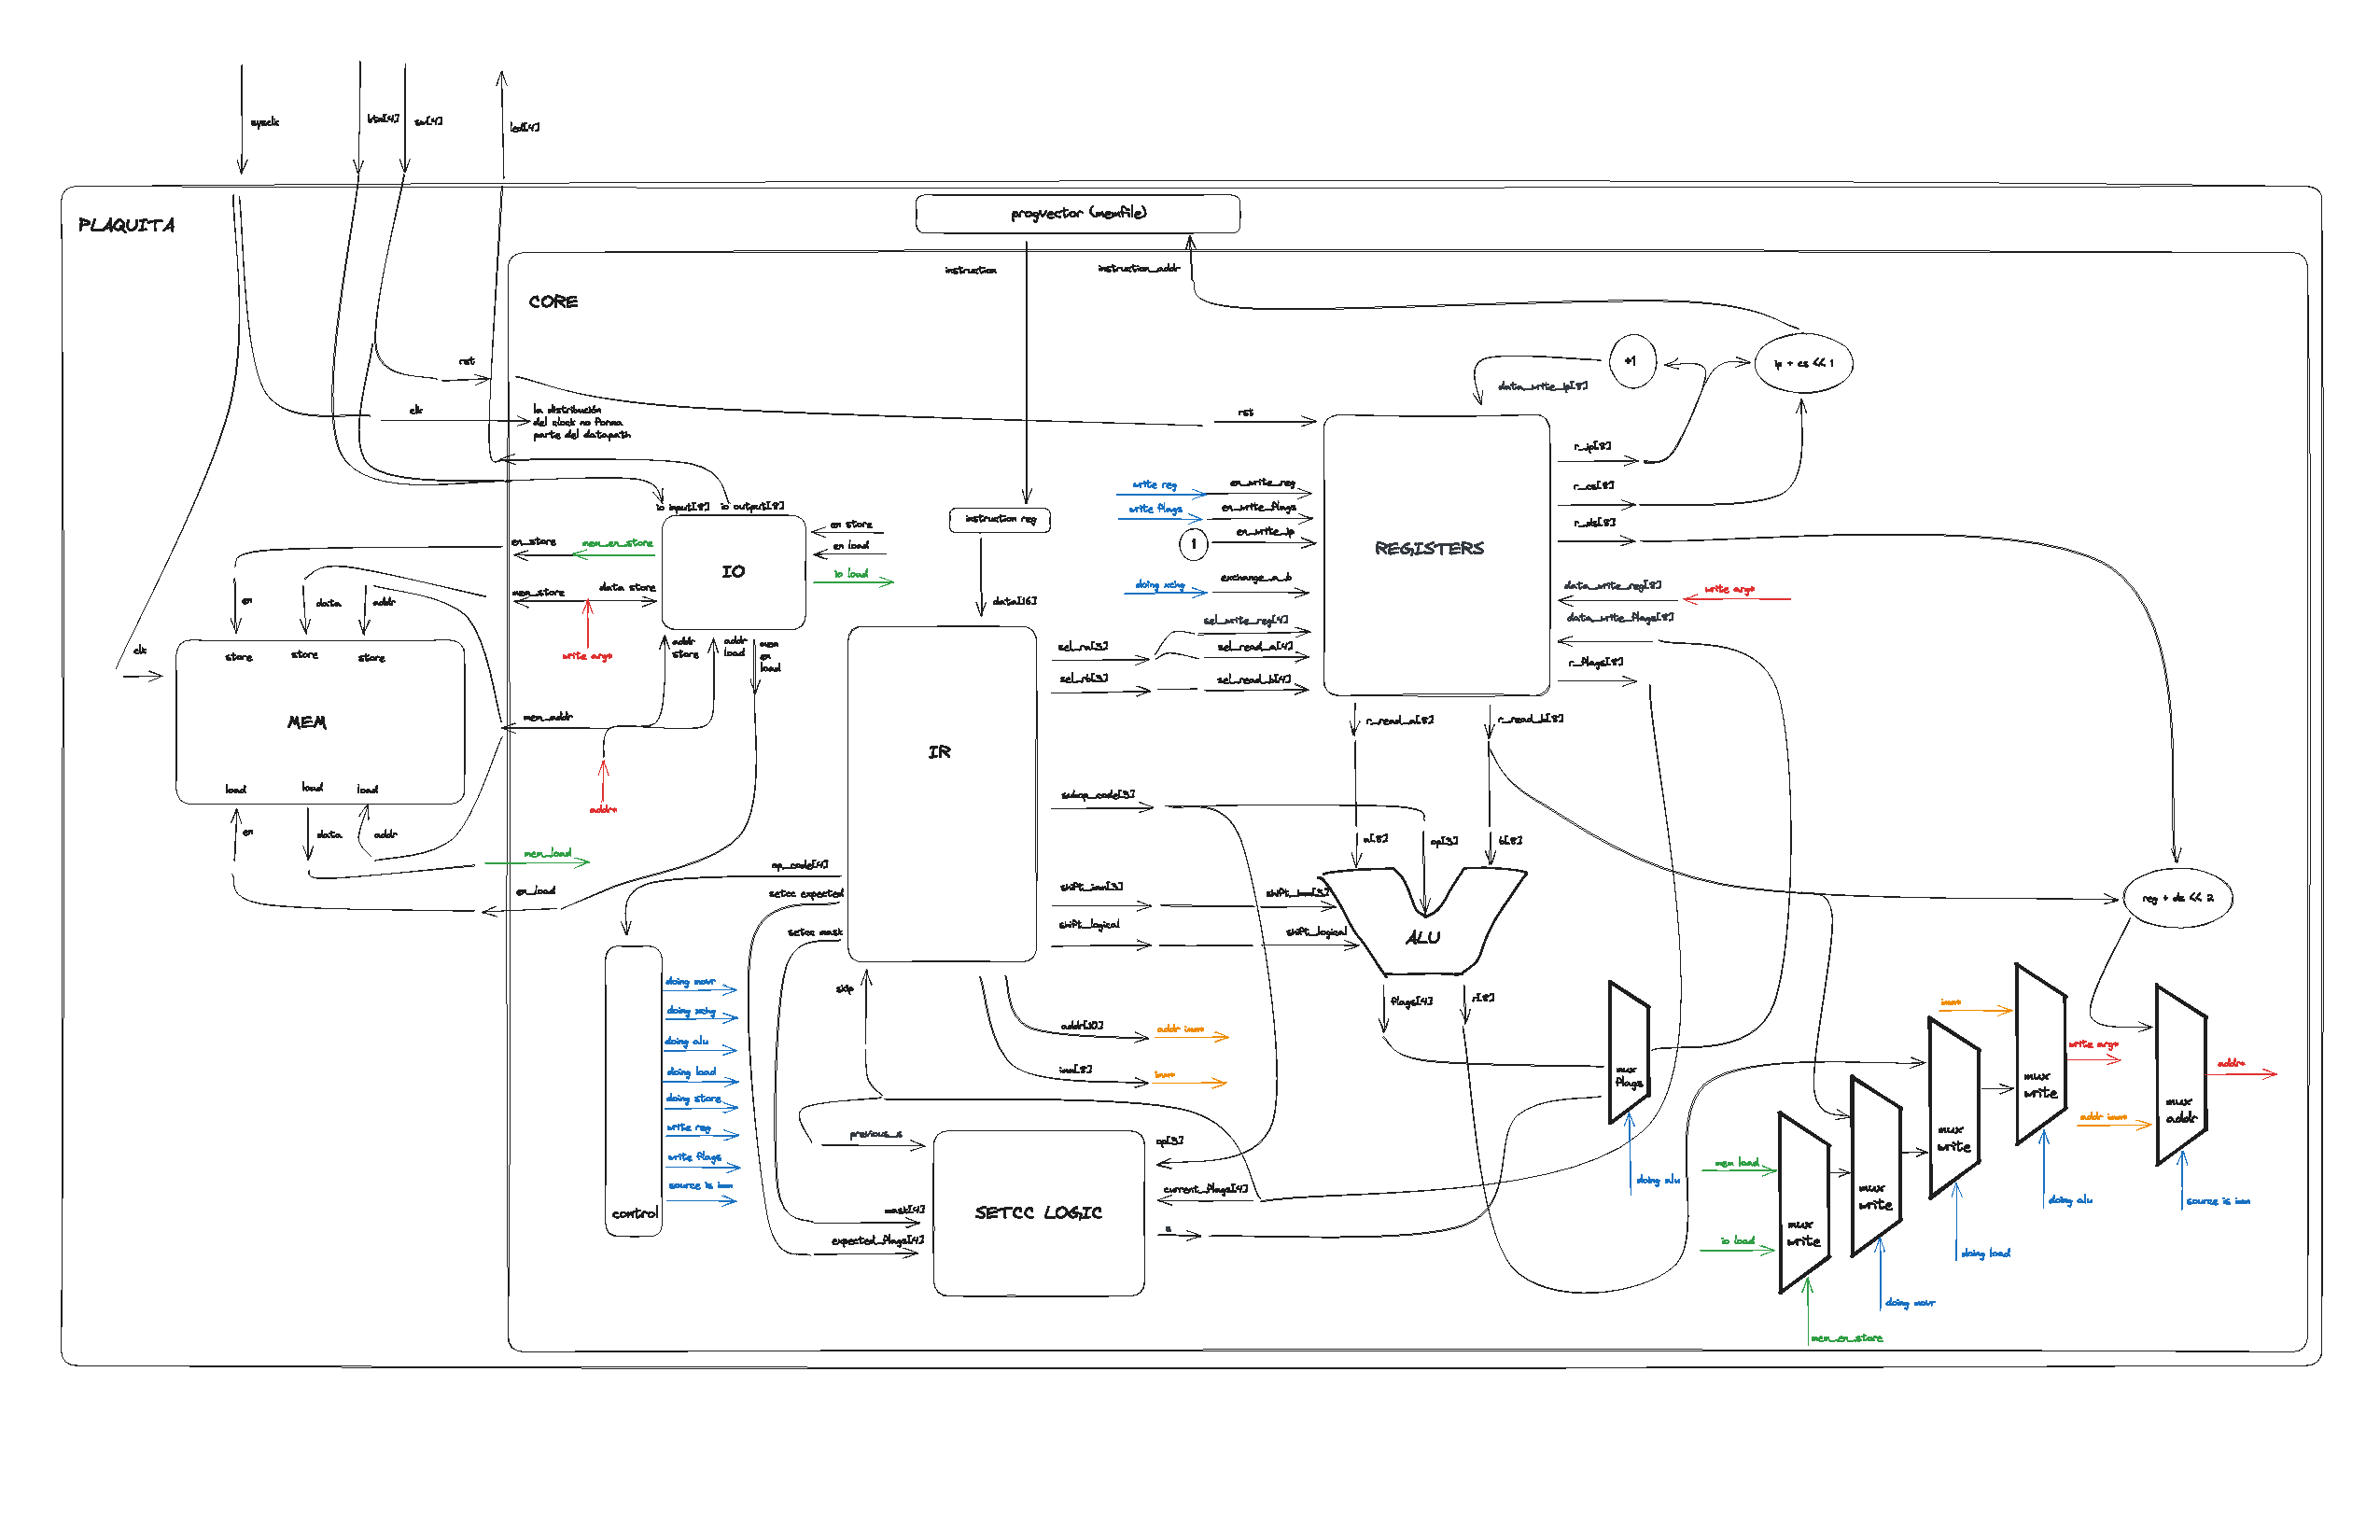
\includegraphics[width=20cm,angle=90]{datapath.pdf}
    \caption{Datapath}
\end{figure}

\newpage

\section{Evaluación}
Cada componente de nuestro procesador (con excepción de \texttt{ir.v} y \texttt{plaquita.v}) tiene un testbench asociado. Cada testbench prueba el componente de manera aislada simulando los estímulos externos que fueran necesarios.
Para la mayoría de los componentes la primera estrategia es adecuada pero \texttt{core.v} requiere de trabajo adicional. La evaluación de \texttt{core.v} se divide en dos testbenchs:
\begin{itemize}
    \item \textbf{core:} Un testbench en el cual se prueba cada instrucción en una cantidad reducida de escenarios. Este testbench todos los estímulos externos (memoria de código y datos) por lo que resulta muy tedioso agregarle tests.
    \item \textbf{progrunner:} Un testbench que realiza una ejecución simulada de un programa dado utilizando una memoria real y una secuencia entradas de I/O esperadas. Este testbench es más fácil de utilizar para verificar el funcionamiento del core, pero no resulta útil como test automatizado ya que no verifica las salidas de I/O.
\end{itemize}

\section{Tooling y ensamblador}
Para escribir programas en nuestra ISA desarrollamos un pequeño ensamblador disponible en \texttt{asm/}. Este ensamblador es un tanto limitado, por lo que utilizamos \texttt{make(1)} para describir un proceso de compilación más útil en el que hacemos uso de \texttt{cpp} como herramienta de preprocesamiento de nuestros archivos. El preprocesamiento nos permite renombrar los registros de forma que el código fuente resulte más fácil de leer.
Como parte de la entrega se incluyen cuatro programas escritos en ensamblador:
\begin{itemize}
    \item \texttt{counter.asm}: Un contador binario que es incrementado luego de apretar un botón de la placa
    \item \texttt{fib.asm}: Cálculo iterativo de números de fibonacci (se visualizan en binario por medio de los leds)
    \item \texttt{random.asm}, \texttt{random-with-sleep.asm}: Generador de números pseudoaleatorio por medio de un \texttt{xorshift} de 16 bits (los números son visibles por medio de los leds)
    \item \texttt{simon.asm}: El juego ``Simon" solicitado por parte de la cátedra
\end{itemize}

\section{Conclusiones y código de ejemplo}

Para cerrar este informe queremos mostrar algunas partes interesantes del código que escribimos durante el desarrollo del trabajo. No consideramos que el diseño (para la ISA, tooling o demos) propuesto sea \emph{``bueno"} pero sí creemos que, además de haber sido una gran experiencia que nos acercó al mundo FPGA, el diseño fué divertido de pensar y construir.

\subsection{Calcular $2^k$ para $k$ pequeño}

Durante el desarrollo del Simon quisimos utilizar un generador de números pseudoaleatorios masomenos realista. Decidimos utilizar un xorshifter con un estado de 16 bits. Un problema con esto es que nosotros queríamos elegir un led al azar (\texttt{0b1000}, \texttt{0b0100}, \texttt{0b0010}, \texttt{0b0001}) pero el generador de números nos otorgaba un número al azar (\texttt{0b00}, \texttt{0b01}, \texttt{0b10}, \texttt{0b11}). En un entorno de desarrollo normal hubiéramos hecho \texttt{1 << n}, pero carecíamos de una operación de shift arbitrario. El poder utilizar el \texttt{ip} como registro de propósito general jugó a nuestro favor, por lo que pudimos escrbir lo siguiente:
\begin{verbatim}
dos_a_la_k:
// input: juanca = k (entre 0 y 7)
// output: juanca = 2^k
    sl juanca 1
    add ip juanca   // saltamos a uno de los movi
    movi juanca 1   // juanca = 0
    ret
    movi juanca 2   // juanca = 1
    ret
    movi juanca 4   // juanca = 2
    ret
    movi juanca 8   // juanca = 3
    ret
    movi juanca 16  // juanca = 4
    ret
    movi juanca 32  // juanca = 5
    ret
    movi juanca 64  // juanca = 6
    ret
    movi juanca 128 // juanca = 7
    ret
\end{verbatim}

\subsection{Un tokenizer es una bolsa de regex}
Para nuestro ensamblador el rendimiento no era muy importante, por lo que decidimos usar los mecanismos más sencillos que encontráramos. A la hora de escribir nuestro \emph{tokenizer} lo caracterizamos por medios de dos tablas (\emph{keywords} y \emph{actionable tokens}. El lexer prueba los patrones uno por uno y ejecuta la acción relacionada al primer match para procesarlo de ser necesario (parseando números, por ejemplo).
\begin{verbatim}
TOKENS_TEXT = {
    # INSTRUCTIONS
    "storei",
    "loadi",
    "movi",
    ...

    # REGISTERS
    "r0",
    ...

    # SIGILS
    "[",
    "]",

    # SETCC
    "zero",
    ...

    # CONDITIONALS
    "maybe",
}

TOKENS_PARSE = [
    # NUMBERS
    (r"0x([0-9a-fA-F]+)",            lambda m: int(m, 16)),
    (r"0b([0-1]+)",                  lambda m: int(m,  2)),
    (r"(\d+)",                       lambda m: int(m, 10)),

    # LABEL DEFS
    (r"([a-zA-Z-_][0-9a-zA-Z-_]+):", lambda m: ('labeldef', m)),

    # SETCC SHENANIGANS
    (r"([cC]?[nN]?[vV]?[zZ]?)",      lambda m: {c.lower(): c == c.upper() for c in m}),

    # LABEL NAMES
    (r"([a-zA-Z-_][0-9a-zA-Z-_]+)", lambda m: ('labelname', m)),
]
\end{verbatim}

\subsection{Parsing por medio de pattern-matching}
Una vez tuvimos el texto tokenizado decidimos parsearlo haciendo uso del pattern-matching presente en las últimas versiones de python. Esto nos permitió expresar las reglas de parseo de forma muy directa.
\begin{verbatim}
def asm_ins(line, labels, is_conditional):
    match line:
        case 'storei', '[', imm10, ']', r4a:
            return asm_store(imm10, r4a)
        case 'loadi', r4a, '[', imm10, ']':
            return asm_load(imm10, r4a)
    
        case 'movi', r4a, imm8: 
            return asm_r4_imm8(0b0111, r4a, imm8, labels=labels)
    
        case 'srl', r4a, imm3: 
            return asm_shift(False, True, is_conditional, imm3, r4a)

        ...
        
        case _:
            raise NotImplementedError(line)
\end{verbatim}

\subsection{La dificultad de escribir loops}
El diseño que dimos para la instrucción \texttt{setcc} no es ideal. La falta de una operación \emph{set} complejiza el código, dado que nos fuerza a ejecutar \texttt{setcc zero} ó \texttt{setcc one} antes de empezar una comparación. Por otra parte, que las instrucciones marcadas con \texttt{maybe} no se ejecuten al setear el bit S resultó poco intuitivo (dado que S=0 nos parecía el estado natural de ese bit). Luego de programar un poco en nuestra ISA la mayoría de los loops tomó la siguiente forma:
\begin{verbatim}
setcc one            // Clear last comparison
loop:
    ...              // Do something
    ...              // Perform a comparison
    setcc and Z      // Check if flags have the proper shape to keep looping
    maybe add ip ONE // If they DONT then exit the loop
    jmpi(loop)       // Otherwise keep looping
//  ^^^^^^^^^^ we cannot `maybe` this because `movi` is not skippable!
\end{verbatim}

\end{document}
